\section{Heterogeneous Computing}
Heterogeneous computing refers to a programming model where multiple different types of computing cores cooporate to solve groups of tasks in an efficient manner \cite{armWhatHeterogenousCompute}.
The \jx is a good example of this; equiped with an 8-core ARM \gls{cpu} and a 512-core NVIDIA \gls{gpu}, as well as several \glspl{asic} including an \gls{isp}, \gls{dla} and two \glspl{nvenc} for specific media encoding and decoding \cite[9, 8, 23, 15-22]{nvidiaNVIDIAJetsonAGX2019}.

This combination of different types of cores working together allows for a system to efficiently handle a wide range of tasks, from general-purpose computing to specialized tasks such as video processing and compression.
This is illustrated in Figure \ref{fig:jx_hierarchy}, where the different types of cores are ordered by their performance and versatility.

While heterogeneous computing systems offer great performance, they also introduce new challenges related to memory management and data transfer between the different types of cores as well as synchronization between the different cores.

\begin{figure}[H]
    \centering
    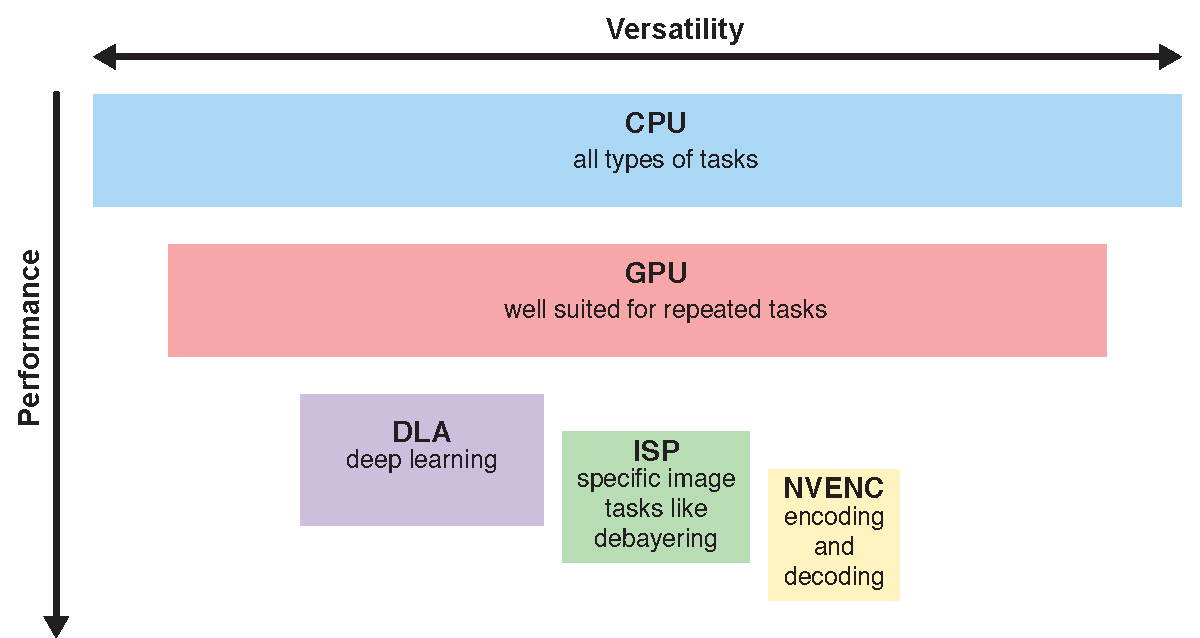
\includegraphics[width=\textwidth]{figures/PDF/jx_hierarchy.pdf}
    \caption{Illustration of the versatility and performance of different types of cores on the \jx.}
    \label{fig:jx_hierarchy}
\end{figure}


\section{GPU programming in CUDA}
In recent years, there has been a significant shift towards parallel computing to enhance processing speed and performance.
\glspl{gpu} have played a vital role in enabling parallel computing across various domains, including machine learning and scientific simulations.
NVIDIA's \gls{cuda} framework and programming model have emerged as a popular platform for parallel computing on \glspl{gpu}.

Programming for \glspl{gpu} differs fundamentally from programming for \glspl{cpu}.
While \glspl{cpu} possess a small number of powerful independent cores, \glspl{gpu} offer a larger number of simpler cores that work collectively on the same task.
This necessitates a distinct code structure to leverage the parallelism provided by \glspl{gpu}.
Additionally, optimizing data movement is crucial due to potential bottlenecks in data transfer between the \gls{cpu} and \gls{gpu}.

A comprehensive explanation of \gls{cuda} is beyond the scope of this thesis.
For more information, the reader is encouraged to refer to the \gls{cuda} Programming Guide \cite{nvidiaCUDAProgrammingGuide} and Volkov's thesis on the topic \cite{volkovLatencyHiding2016}.
Nevertheless, the subsequent sections present key concepts relevant to this thesis.

\subsection{CUDA hierarchy}
The basic unit of execution in \gls{cuda} is the kernel, which is a function that is executed on the \gls{gpu} \cite[11]{nvidiaCUDAProgrammingGuide}.
A kernel is executed by a grid of blocks, where each block is executed by a group of threads.
This is illustrated in Figure \ref{fig:cuda_hierarchy}.

A block represents a cluster of threads that can be scheduled to run concurrently on a \gls{sm} of the \gls{gpu}.
Threads within a block can synchronize their execution to coordinate memory accesses and collaborate by utilizing shared memory, which is a fast but limited resource \cite[13,19]{nvidiaCUDAProgrammingGuide}.

Threads are executed in warps, which are groups of 32 threads.
Within a warp, threads execute the same instruction simultaneously, while different warps can execute distinct instructions in parallel \cite[10-12]{volkovLatencyHiding2016}.
However, if threads within a warp follow different execution paths, such as when encountering an \code{if} statement, the warp will execute both paths sequentially, resulting in reduced performance due to warp divergence \cite[10-12]{volkovLatencyHiding2016}.

\begin{figure}[H]
    \centering
    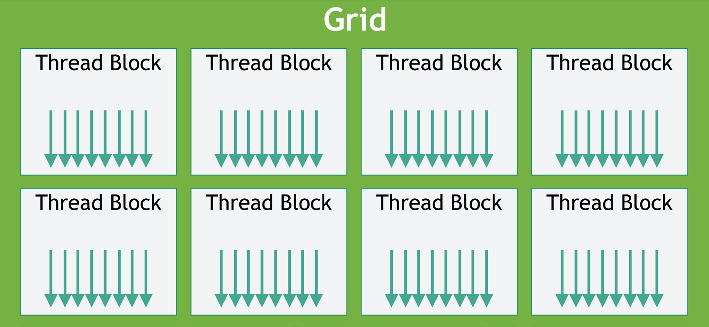
\includegraphics[width=.6\textwidth]{figures/concurrency/cuda_hierarchy.pdf}
    \caption{Grit of Thread Blocks \cite[15]{nvidiaCUDAProgrammingGuide}.}
    \label{fig:cuda_hierarchy}
\end{figure}

\subsubsection{Latency Hiding}
Latency hiding is a technique used by modern commodity processors such as \glspl{gpu} to better utilize their numerous execution units and hide execution latencies \cite[35]{volkovLatencyHiding2016}.
The idea behind latency hiding is to keep the processor busy with other tasks while it waits for data to be fetched from memory.
This is achieved by executing multiple threads in parallel, so that when one thread is waiting for data, another thread can continue executing, as illustrated in Figure \ref{fig:concurrency}.

\begin{figure}[H]
    \centering
    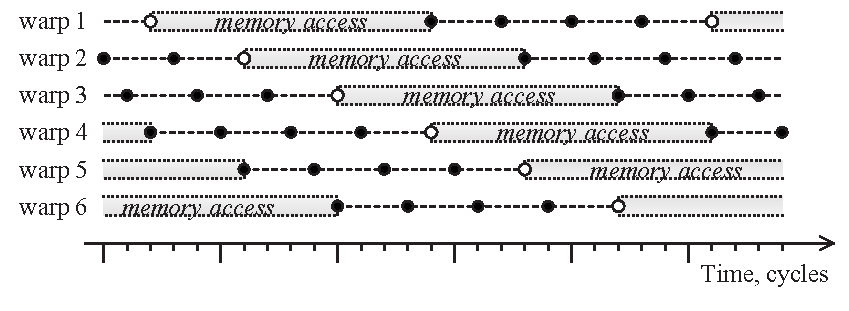
\includegraphics[width=.7\textwidth]{figures/PDF/concurrency_p54.pdf}
    \caption{Visualization of concurrent execution on a GPU \cite[54]{volkovLatencyHiding2016}}
    \label{fig:concurrency}
\end{figure}



\section{Memory management on Jetson platform}
\label{sec:jx_memory}
On \gls{tegra} platforms, there are different types of memory available for use, including device memory, pageable host memory, pinned memory, and unified memory \cite[13]{nvidiaCUDAFTegra2023}.
These memory types are allocated on the same physical DRAM but have different accessing and caching behaviors \cite[5]{nvidiaCUDAFTegra2023}.
A summary of the different memory types is presented in Table \ref{tab:memory_types}.


\providecommand{\tmpfootnote}{\footnote{Cached where compute capability is greater than or equal to 7.2 \cite{nvidiaCUDAFTegra2023}. The \jx has compute capability of 7.2 \cite{CUDA2023}}}

\begin{table}[H]
    \centering
    \begin{tabular}{ |c|c|c| }
        \hline
        \textbf{Memory Type} & \textbf{CPU}            & \textbf{gpu}            \\
        \hline
        Pageable host memory & Cached                  & Not directly accessible \\
        Device memory        & Not directly accessible & Cached                  \\
        Pinned host memory   & Cached                  & Uncached                \\
        Pageable host memory & Cached \tmpfootnote     & Cached                  \\
        \hline
    \end{tabular}
    \caption{Memory types on the \jx \cite{nvidiaCUDAFTegra2023}}
    \label{tab:memory_types}
\end{table}

\paragraph{Pageable host memory} is equivalent to \gls{cpu} memory on normal computers.
When memory is pageable the \gls{cpu} can control where it is stored, and it can be moved to the \gls{swap} area to free up physical memory \cite[6]{nvidiaCUDAFTegra2023}.
This makes in unacessable by the \gls{gpu}.

\paragraph{Device memory} refers to the memory that can be directly accessed by the \gls{gpu} but not by the \gls{cpu} \cite[5]{nvidiaCUDAFTegra2023}. It is allocated on the same physical DRAM as other memory types but cached in a manner optimized for \gls{gpu} usage, rendering it inaccessible to the \gls{cpu} \cite[5]{nvidiaCUDAFTegra2023}.

\paragraph{Pinned host memory}, also referred to as page-locked memory, enables direct access by both the \gls{cpu} and the \gls{gpu} in Tegra systems, eliminating transfer overhead \cite[9]{nvidiaCUDAFTegra2023}.
Unlike device memory, pinned host memory is not cached on the \gls{gpu}, making it less efficient for repeated data access \cite[9]{nvidiaCUDAFTegra2023}.

\subsubsection{Unified memory} is accessible and cached on both the \gls{gpu} and the \gls{cpu}, making it a suitable choice for memory that is repeatedly accessed from both devices \cite[10]{nvidiaCUDAFTegra2023}. However, unified memory incurs additional overhead compared to pinned memory \cite[12]{nvidiaCUDAFTegra2023}.